% Created 2018-10-13 Sa 17:05
% Intended LaTeX compiler: pdflatex
\documentclass[11pt]{article}
\usepackage[utf8]{inputenc}
\usepackage[T1]{fontenc}
\usepackage{graphicx}
\usepackage{grffile}
\usepackage{longtable}
\usepackage{wrapfig}
\usepackage{rotating}
\usepackage[normalem]{ulem}
\usepackage{amsmath}
\usepackage{textcomp}
\usepackage{amssymb}
\usepackage{capt-of}
\usepackage{hyperref}
\author{Nikolai Weidt}
\date{\today}
\title{Calcback}
\hypersetup{
 pdfauthor={Nikolai Weidt},
 pdftitle={Calcback},
 pdfkeywords={},
 pdfsubject={},
 pdfcreator={Emacs 26.1 (Org mode 9.1.14)}, 
 pdflang={English}}
\begin{document}

\maketitle
\tableofcontents

\bibliography{forschungspraktikum}
\section{What is this?}
\label{sec:org1000554}
I'm coding a program to get the complex refractive index \(n = n * ik\) from the ellipsometric parameters \(\Delta\) and \(\Psi\) I got from a simulation.
\section{Imports:}
\label{sec:org17d5ecd}
\begin{verbatim}
import numpy as np
import matplotlib
from matplotlib import pyplot
\end{verbatim}

\section{Defining some variables:}
\label{sec:org00ef83b}
Defining some variables for later use:

\begin{verbatim}
CSVFILE = "head300nmSiO2.csv"
phi_i = 70 * np.pi / 180
d_L = 300
n_air = 1
rerange = 5
imrange = 5
i = 0
\end{verbatim}

\section{Read .csv-file:}
\label{sec:org26419b9}
Read the values into a two dimensional numpy array as [[lambda,Psi,Delta,n\(_{\text{S,k}}\)\(_{\text{S}}\)],\ldots{}] (Skip columns 3 and 4)

\begin{verbatim}
csv = np.loadtxt(CSVFILE, usecols=(0,1,2,5,6),  delimiter=",", skiprows=1)
\end{verbatim}

:DEBUG:
The array looks like this:
\begin{verbatim}
print(csv)
\end{verbatim}
\begin{center}
\begin{tabular}{rrrrr}
300 & 55.2217535 & 84.37228319 & 2.6726 & 3.0375\\
303 & 50.11187439 & 93.3085011 & 2.7346 & 3.0381\\
306 & 46.35824553 & 98.43681392 & 2.7967 & 3.0368\\
309 & 43.50539341 & 101.18051798 & 2.8588 & 3.0334\\
312 & 41.29392865 & 102.19236832 & 2.9206 & 3.0279\\
315 & 39.48751217 & 101.93002 & 2.9822 & 3.0205\\
318 & 37.90308303 & 100.64846104 & 3.0435 & 3.0109\\
321 & 36.47640803 & 98.54577151 & 3.1042 & 2.9994\\
324 & 35.12615859 & 95.72242205 & 3.1644 & 2.9858\\
\end{tabular}
\end{center}

\section{Calculate \(\rho\)}
\label{sec:org7a5acd2}
\subsection{Create a matrix containing every possible refractive index (n+ik):}
\label{sec:org77978a0}
\begin{verbatim}
lsp_re = np.linspace(0.1, rerange, 101)
lsp_im = np.linspace(0.1, imrange, 101)
re, im = np.meshgrid (lsp_re, lsp_im, copy=False)
matrix = 1j * im + re
\end{verbatim}

This gives the following matrix:
\begin{verbatim}
print(matrix)
\end{verbatim}

\begin{verbatim}
[[0.1  +0.1j   0.149+0.1j   0.198+0.1j   ... 4.902+0.1j   4.951+0.1j
  5.   +0.1j  ]
 [0.1  +0.149j 0.149+0.149j 0.198+0.149j ... 4.902+0.149j 4.951+0.149j
  5.   +0.149j]
 [0.1  +0.198j 0.149+0.198j 0.198+0.198j ... 4.902+0.198j 4.951+0.198j
  5.   +0.198j]
 ...
 [0.1  +4.902j 0.149+4.902j 0.198+4.902j ... 4.902+4.902j 4.951+4.902j
  5.   +4.902j]
 [0.1  +4.951j 0.149+4.951j 0.198+4.951j ... 4.902+4.951j 4.951+4.951j
  5.   +4.951j]
 [0.1  +5.j    0.149+5.j    0.198+5.j    ... 4.902+5.j    4.951+5.j
  5.   +5.j   ]]
\end{verbatim}
\subsection{Calculate:}
\label{sec:org475c76a}
\subsubsection{By using Snell's Law to calculate the refractive angles inside the media.}
\label{sec:org464757d}
Phi is the incident angle for the layer, n1 and n2 are refractive indices of first and second medium. Returns the angle of refraction.

\begin{figure}[htbp]
\centering
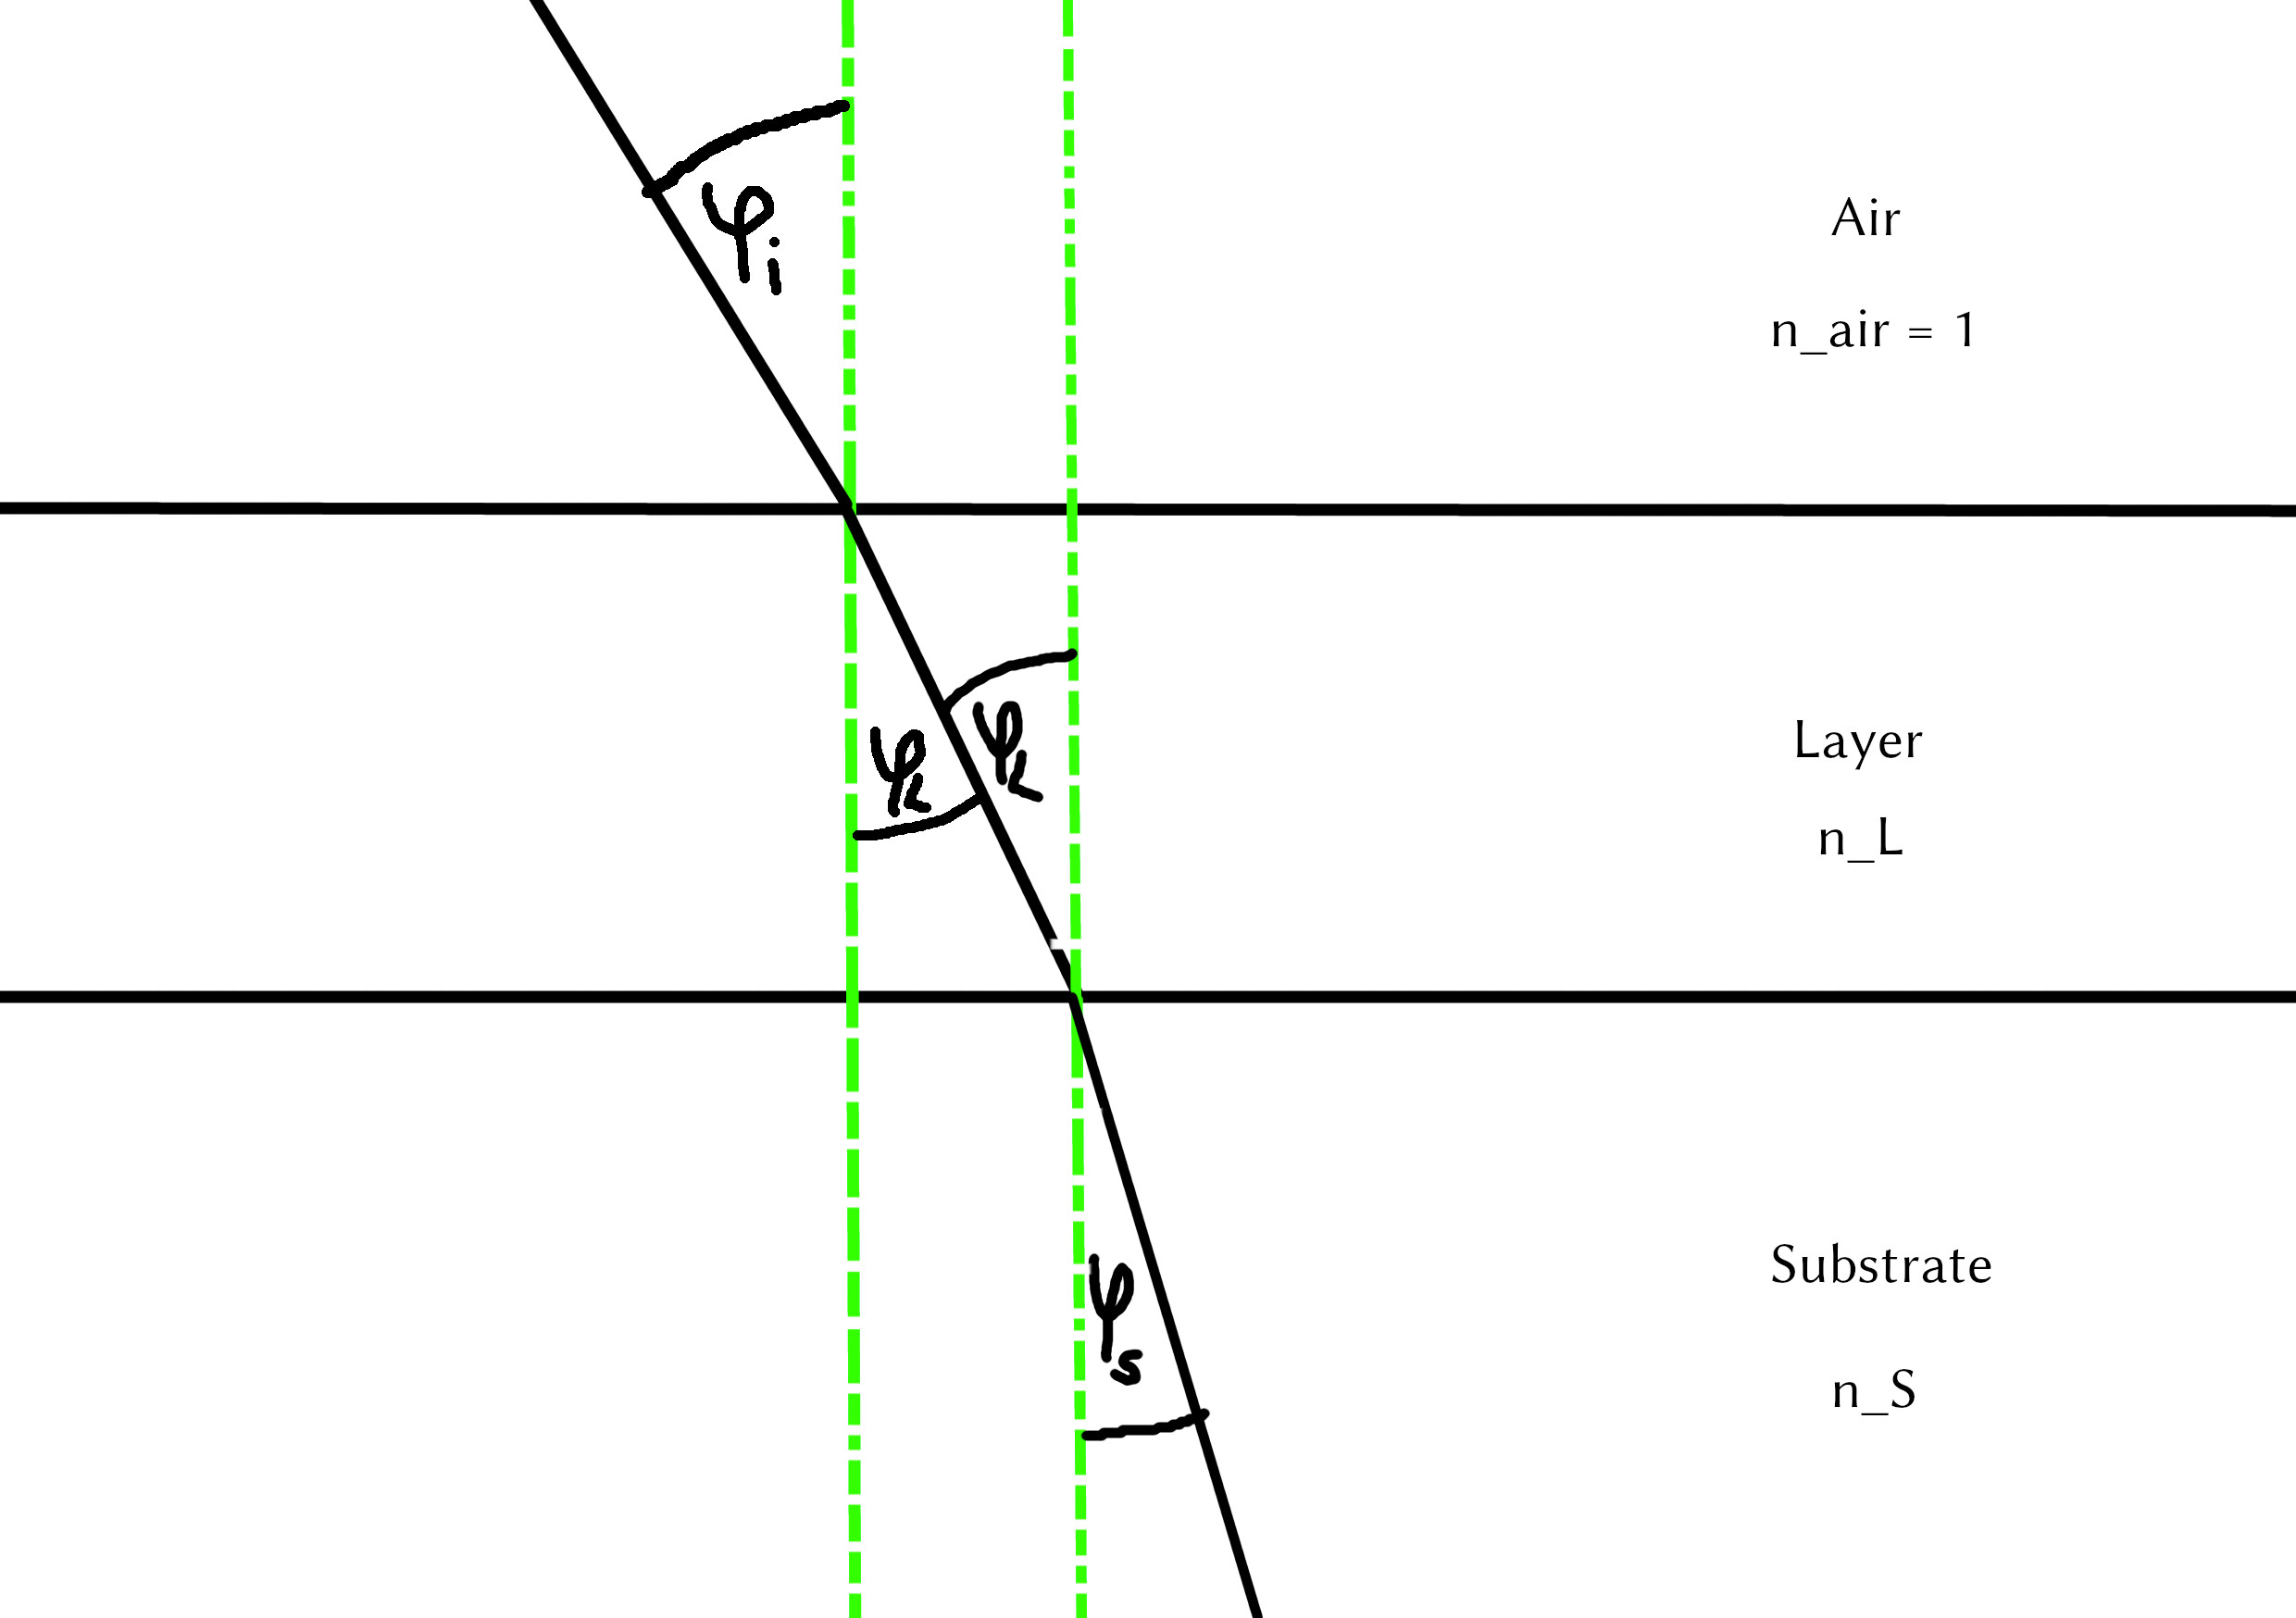
\includegraphics[width=500]{./snell.jpg}
\caption{\label{fig:orgad8beb4}
Snell's Law}
\end{figure}
\begin{verbatim}
def snell(phi, n1, n2):
    phi_ref = np.arcsin((np.sin(phi) * n1) / n2)
    return phi_ref
\end{verbatim}


\subsubsection{{\bfseries\sffamily TODO} Calculate r\(_{\text{p}}\) and r\(_{\text{s}}\) with Fresnel equations:}
\label{sec:orga262a86}
\begin{verbatim}
def fresnel(n1, phi1, n2, phi2):
    return rs, rp
\end{verbatim}

\subsubsection{{\bfseries\sffamily TODO} Calculate \(\rho\) after Fujiwara \cite{fujiwara2009spectroscopic}:}
\label{sec:orgdfd9357}
\subsubsection{{\bfseries\sffamily TODO} Wrap a for-loop around these functions to calculate \(\rho\) for every n\(_{\text{L}}\) in the matrix}
\label{sec:org198c2e1}
\begin{verbatim}
n_S = (csv[i,3] + 1j* csv[i,4])
lambda_vac = csv[i,0]
for n_L in matrix.flat:
      phi_L = snell(phi_i,n_air,n_L)
      phi_S = snell(phi_L,n_L,n_S)
      # Fresnel equations:
      #
      # air/layer:
      rs_al = (n_air * np.cos(phi_i) - n_L * np.cos(phi_L)) / (n_air * np.cos(phi_i) + n_L * np.cos(phi_L))
      rp_al = (n_L * np.cos(phi_i) - n_air * np.cos(phi_L)) / (n_L * np.cos(phi_i) + n_air * np.cos(phi_L))
      # layer/substrate:
      rs_ls = (n_L * np.cos(phi_L) - n_S * np.cos(phi_S)) / (n_L * np.cos(phi_L) + n_S * np.cos(phi_S))
      rp_ls = (n_S * np.cos(phi_L) - n_L * np.cos(phi_S)) / (n_S * np.cos(phi_L) + n_L * np.cos(phi_S))
      # Fujiwara:
      beta = 2 * np.pi * d_L * n_L * np.cos(phi_L) / lambda_vac
      rp_L = (rp_al + rp_ls * np.exp(-2*1j*beta)) / (1 + rp_al * rp_ls * np.exp(-2 * 1j * beta)) 
      rs_L = (rs_al + rs_ls * np.exp(-2*1j*beta)) / ( 1 + rs_al * rs_ls * np.exp(-2 * 1j * beta))   
      rho = rp_L / rs_L
      output = []
      output.append([n_L, rho])
\end{verbatim}


\begin{verbatim}
for n_L =  (5+5j)
at lambda =  300.0
phi_L (0.09369049752311029-0.0942436309601521j)
phi_S (0.1516718935900151-0.1754940397472108j)
rs_al (-0.9322788656900732-0.06447800755339925j)
rp_al (0.47076999129408226+0.32915273622391117j)
rs_ls (0.2706645644366405-0.037805743704596925j)
rp_ls (-0.27413124901624036+0.021323198111731292j)
beta (31.139752412112067+31.69455000949363j)
rp_L (1.426723122645158-0.9975355870956931j)
rs_L (-1.067534044700266+0.07383248803644696j)
rho (-1.3944229215529675+0.8379890813445299j)
output [[(5+5j), (-1.3944229215529675+0.8379890813445299j)]]
\end{verbatim}

\subsection{Compare calculated rho with given \(\Delta\) and \(\psi\):}
\label{sec:orgb28adba}
\end{document}